\chapter*{Svalbard}\\ {\footnotesize \textit{08--20 mars}}

\begin{figure}[H]
	\centering
\noindent\makebox[\textwidth]{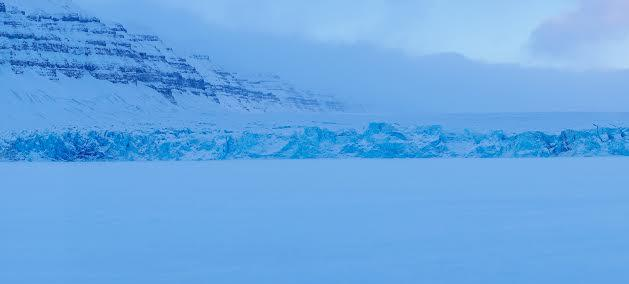
\includegraphics[width=6.125in]{tunaglaciervenstre}}
	\caption*{}
\label{fig:venstre}
\end{figure}
\textbf{Om du tror Svalbard minner om det norske høyfjellet tar du feil.
Svalbard gikk aldri ut av istiden.
Isen
her er gammel.  Veldig gammel. I 20000 år har isen vært her.} 

\chapter*{\\ \\}\\ {\footnotesize \textit{\\ \\ \\ \\ \\ \\ \\ \\ \\ \\ \\ \\ }}
\begin{figure}[H]
	\centering
\noindent\makebox[\textwidth]{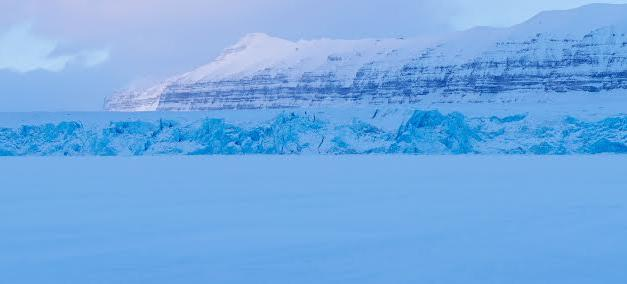
\includegraphics[width=6.125in]{tunaglacierhoyre}}
	\caption*{}
\label{fig:venstre}
\end{figure}
\textbf{Den samme isen som
slepet det norske grunnfjellet til fjorder og daler. Her smeltet den
aldri. Den kjemper en evig kamp mot det arktiske havet som uavbrutt slår inn i alle ender. Å se denne isfronten på nært hold kan
verken beskrives med mine ord eller bilder.}


